\documentclass[10pt, a4paper]{article}

\usepackage{amsmath}
\usepackage{amssymb}
\usepackage{graphicx}
\usepackage{listings}
\usepackage{color}
\usepackage[section]{placeins}
\usepackage{paralist}

\definecolor{mygreen}{rgb}{0,0.6,0}
\definecolor{mygray}{rgb}{0.5,0.5,0.5}
\definecolor{mymauve}{rgb}{0.58,0,0.82}

\lstset{ %
  backgroundcolor=\color{white},
  basicstyle=\footnotesize,
  breakatwhitespace=false,
  breaklines=true,
  captionpos=b,
  commentstyle=\color{mygreen},
  escapeinside={\%*}{*)},
  extendedchars=true,
  keepspaces=true,
  keywordstyle=\color{blue},
  rulecolor=\color{black},
  showspaces=false,
  showstringspaces=false,
  showtabs=false,
  stepnumber=2,
  stringstyle=\color{mymauve},
  tabsize=2,
}

\hyphenation{GENITOR}

\newcommand*{\titleGM}{\begingroup
\hbox{ 
\hspace*{0.2\textwidth} 
\rule{1pt}{\textheight} 
\hspace*{0.05\textwidth} 
\parbox[b]{0.75\textwidth}{ 

{\noindent\Huge\bfseries Genetic Algorithms}\\[2\baselineskip] % Title
{\large \textit{SEM6120 - Assignment 1}}\\[4\baselineskip] % Tagline or further description
{\Large \textsc{Alexander D Brown (adb9)}} % Author name

\vspace{0.5\textheight} 
}}
\endgroup}


\title{Genetic Algorithms}
\author{Alexander D Brown (adb9)}

\begin{document}
\titleGM 
\tableofcontents

\newpage
\section{Introduction}
Genetic algorithms are a biologically-inspired approach to heuristic search 
that mimic natural selection. Unlike many other evolutionary strategies and
evolutionary programming, they are not designed to solve a specific problem,
but are designed to solve the problem of optimisation which is made difficult
by substantial complexity and uncertainty\cite{Holland1992Adaptation}.

The complexity of the task should make it such that discovering an optimum
solution is a long, maybe even impossible, task. At the same time the 
uncertainty needs to be reduced so that the knowledge of \textit{available}
options can be increased.

% TODO improve this section as its mainly from the reference.
The initial design for a genetic algorithm was a method for moving from one
population of chromosomes to another using a form of natural selection. This
algorithm also included methods for crossover, mutation and inversion. This
idea of having a large population was the distinguishing feature from any past
attempts which had only considered the parent and one offspring, where the 
offspring was simply a mutation of the parent\cite{Mitchell1996Introduction}.


\subsection{Evolutionary Algorithms}
As their name suggests, an evolutionary algorithm applies elements from the 
biological theory of evolution to the problem of optimisation. These elements
include:

\begin{itemize}
\item Reproduction
\item Mutation
\item Recombination
\item Selection
\end{itemize}

Typically, a population of candidate solutions are generated to which a fitness
function can be applied. The population is then subject to some form of 
evolution, and this process is repeated until a halting criteria is met.

Genetic algorithms are a type of evolutionary algorithm with a focus on the 
genetic evolution of solutions. Candidate solutions for genetic algorithms, 
known as \textit{chromosomes} are encoded as a series of \textit{genes}. These
genes are a representation of the choices which need to be optimised for the 
solution and can be as simple as a single bit or as complex as a real number, 
depending on the problem.

There are many other forms of both evolutionary and genetic algorithms which
this report with mention in later sections.


\subsection{Genetic Algorithms}
The basic principals of genetic algorithms are to represent candidate solutions
as a population of chromosomes, from this population the fittest members can be
picked out and used in the next generation and to create new member of the 
population through reproduction and/or mutation.

This cycle repeats with the aim to produce better performing individuals in 
each generation until the optimum solution is either reached or gotten close
enough to that any future improvement is unnecessary or unwanted due to
other constraints such as processing time. The latter of these allows a genetic
algorithm to come up with a ``good'' solution in a reasonable amount of time.

Reproduction and mutation are an important part of genetic programming, and too
of evolutionary programming. Without these parts the algorithm would quickly 
reach a local optimum for the initial population and would not improve past 
this.

\subsection{Chromosome Representation}
One of the key parts parts in implementing a genetic algorithm is the 
representation of chromosomes. This is very dependent of the problem the 
genetic algorithm needs to optimise and can have a knock on affect on the 
efficiency and accuracy of the algorithm.

Sometimes a simple solution is enough to represent the problem, binary strings
are a commonly suggested approach. However sometimes more complex 
representations are required, potentially any data structure can be used as a
chromosome but lists and trees are the common choices as they are easy to 
perform crossover\footnote{A term used instead of reproduction in genetic 
algorithms.} and mutation on.

As a very simple example, to maximise $y$ in: $y = f(x)$, one could represent 
the value of $x$ as a binary string, an example of which is shown in 
figure~\ref{fig:chromosome}.

\begin{figure}[h]
\centering
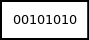
\includegraphics[scale=0.6]{img/chromosome.png}
\caption{Chromosome representation as a binary string}\label{fig:chromosome}
\end{figure}

\subsection{Fitness Function}
To fulfil the step of natural selection; the process of choosing the ``best''
members of a population, there needs to be a way of evaluating each chromosome,
such that they can be compared to one another.

The function for doing so is known as a fitness function, which typically 
returns either a single number or a list of numbers, depending on the problem.
Each chromosome can then be ranked in order of fitness and the top members of
a population can then be selected.

As the value returned from a fitness function, with be specific to the domain 
it has be used within, it is necessary to rescale the fitness value to ensure 
uniformity when genetic algorithms are applied over several different domains
at the same time. %TODO citation needed.


\subsection{Selection}
Selection simulates the ``survival of the fittest'' nature of biology. However,
it is beneficial not to keep some lesser performing members of the population
to avoid getting trapped in local optimum. Most selection algorithms will 
introduce an element of randomness into the selection to deal with this.

Simple methods for selection typically involve randomly selecting individuals,
giving those individuals with higher fitness greater chance of being selected.
While others take inspiration from biology by making members of the population
complete or assign individuals genders to imitate sexual reproduction.

\subsection{Crossover}
% Talk about methods of crossover
% - Crossover point
% - Mask-based crossover
% - Other strategies (sexual, etc.) 

Crossover is the algorithmic approach to replicating biological reproduction
and is key to genetic algorithms as it will produce new, unseen, offspring
based on selected members of the population.

In its simplest form crossover is the process of taking one chromosome and
splicing it with another. This can be done in several ways, but the most common
is to choose a random point, known as the \textit{crossover point}. The
offspring consists of all the genes from the first parent up until the 
crossover point, the remaining genes then come from the second parent. As shown
in figure~\ref{fig:crossover-point}.

\begin{figure}[h]
\centering
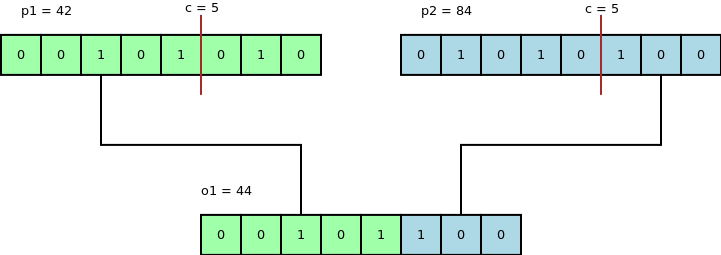
\includegraphics[scale=0.45]{img/crossover.png}
\caption{Crossover of parents $p1$ and $p2$ at crossover point $c$, where 
         $c=5$, resulting in offspring $o1$.} 
\label{fig:crossover-point}
\end{figure}

More complex methods revolve around the idea of having multiple crossover 
points and eventually it becomes more efficient to use a binary mask over
the two parents, as shown in figure~\ref{fig:crossover-mask}

\begin{figure}[h]
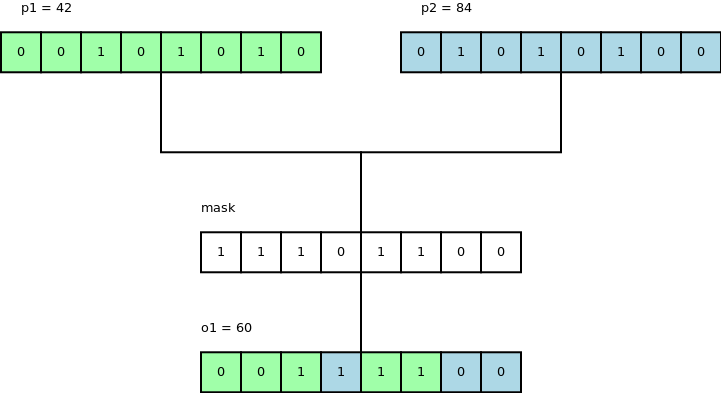
\includegraphics[scale=0.45]{img/mask-crossover.png}
\caption{Crossover of parents $p1$ and $p2$ using a binary mask, resulting in
         offspring $o1$}
\label{fig:crossover-mask}
\end{figure}

This can lead to problems if the representation of chromosomes is complex; if,
for example, each gene represents a node in the travelling salesman problem
then crossover can produce routes which are invalid as nodes may be duplicated
due to this process.

\subsection{Mutation}
% Talk about methods of mutation
% - Flipping bits/values

Another method of getting variation into a population is mutation, the random
change of genes within a chromosome. In genetic algorithms this is typically
replicated by flipping a single bit in the chromosome.

As with crossover, mutation must be handled carefully with complex chromosome
representations as it may lead to invalid chromosomes. The rate of mutation 
is usually kept low to avoid large amounts of variance.


\subsection{Termination}
% Talk about termination criteria

The final problem with genetic algorithms is the problem of deciding when a 
result is good enough. Usually the implementation has some form of termination
criteria, this may be a time limit or number of generations or may be something
more complex like when the algorithm no longer improves in fitness greatly.

Termination criteria is very specific to the problem domain. Genetic algorithms
are very good at giving an approximate answer and typically bad at finding the
exact optimum solution.

\FloatBarrier

\newpage
\section{Previous Research into Selection Schemes}
\label{sec:selection-algorithms}

This report focuses on reviewing previous research into selection schemes,
focusing mainly on analysis of commonly used selection schemes through a range
of methods, as well as viewing some more advanced techniques which are being
used in recent years.

This section will briefly introduce each paper to give a general overview on
each. The following section will then go on to critically evaluate each paper
and start to draw conclusions on the research done.

\subsection{A Comparative Analysis of Selection Schemes used in Genetic Algorithms}
\subsubsection{Introduction} 
There have been studies into the effects of different selection algorithms on 
genetic algorithms. Goldberg and Deb\cite{Goldberg1991Comparative} compared
four methods of selection; proportional reproduction, ranking selection,
tournament selection and the GENITOR algorithm\cite{Whitley1989GENITOR}.

%TODO More introduction to this.

\subsubsection{Comparison Techniques} 
Selection schemes were analysed in terms of:

\begin{enumerate}
\item Growth ratio; the expected ratio for the members of the best class to the
umber of members of the population.
\item Takeover time; the approximate number of generations it takes
to converge, this gives an idea of how long it would take before mutation,
rather than crossover, becomes the primary method for exploring the search
space. 
\item Time complexity using the standard big O measure.
\end{enumerate}

These values were chosen to allow side-by-side comparison of each selection
scheme and help to provide useful information as to which scheme might be
correct for a certain scenario.

The growth ratio is defined in three points of generation;
\begin{inparaenum}[1\upshape)]
\item at generation $t$ ($\phi_t$),
\item when the proportion of individuals is is insubstantial (the \textit{early}
      ratio - $\phi_e$) and
\item when the best individual occupies 50\% of the population (the
      \textit{late} ratio - $\phi_l$).
\end{inparaenum}

These values are picked to give an idea of the performance in a general case for
$\phi_t$; towards the beginning of convergence at $\phi_e$, where growth rates
are typically high and towards the end of convergence at $\phi_l$ where growth
rates are expected to be low.

\subsubsection{Results} 
Linear ranking and binary tournament (a tournament with a pool size of two
individuals) were found to have similar growth rates. Tournaments selection
could produce better growth rates simply through larger pool sizes, whereas
ranking selection would need a non-linear function, making them more expensive
to implement and run.

Takeover times all converged in around $O(log\;n)$ generations. This is not at
all surprising, given that the problem space only has a single optimum point.
The authors note that this will not be the convergence of a real GA. The results
of takeover time should be used to determine a rough estimate for when mutation,
and not crossover, becomes the primary method of exploration.

Most interestingly the time complexities had a large range, from $O(n^2)$ to 
$O(n)$, with tournament selection being an $O(n)$. This is particularly 
interesting as tournament selection is a very easy algorithm to make parallel,
this fits in with genetic algorithms nicely as they improve drastically from 
parallel implementation.

\subsection{Genetic Drift in Selection Schemes}
\subsubsection{Introduction} 
Rogers and Pr\"{u}gel-Bennett\cite{Rogers1999Genetic} defined a method of 
analysing selection schemes using genetic drift, a term borrowed from biology,
which describes the change in frequency of an allele (gene variation) through
random sampling of the population.

Genetic drift is a phenomenon observed in genetic algorithms due to the nature
of selection and, unlike analysis methods like convergence time, leads to a
exact analytical solution. Though previous attempts to calculate genetic drift
were often approximations or difficult to generalise to other cases, according
to the authors.

\subsubsection{Genetic Drift} 
In genetic algorithms, genetic drift is a measure of the change in fitness
variation within a population and is worked out using probabilistic analysis of
the selection scheme. 

To analyse genetic drift, the variation of population fitness needs to be
calculated. Standard variance ($\sigma^2$) is applied to the initial population
of $P$ members. Each member ($\alpha$) has fitness $F_\alpha$. Therefore the
variance is defined as:

\begin{equation}
\sigma_F^2 = \text{E}[F^2] - (\text{E}[F])^2
\end{equation}

Calculating this out becomes:

\begin{equation}
\sigma_F^2 = \frac{1}{P}\sum^{P}_{\alpha=1}{F^{2}_{\alpha}} - \left(
\frac{1}{P}\sum^{P}_{\alpha=1}{F_{\alpha}}\right)^2
\end{equation}

Applying a selection scheme to this population and drawing a new population of
$P$ individuals means there will be $n_\alpha$ copies of a population member
$F_\alpha$. The variance of the new population is given as:

\begin{equation}
\sigma'^2_F = \frac{1}{P} \sum^{P}_{\alpha=1}{n_\alpha F^2_\alpha} - \left(
\frac{1}{P} \sum^P_{\alpha=1}{n_\alpha F_\alpha}\right)^2
\end{equation}

To get an average case the authors averaged over all the possible ways of
performing selection. To do this they looked at neutral selection, where the
probability of selection is due to random, neutral, occurrences and not due to
any form of fitness of the individual. This allows $n_\alpha$ to be independent
of $F_\alpha$. By working through this and simplifying further to use the fact
that $P$ is kept constant, they derive:

\begin{equation}
\text{E}[\sigma'^2_F] = \frac{P - \text{E}[n^2]}{P-1}\sigma^2_F
\label{eq:average-case}
\end{equation}

The change in population fitness variance for any selection scheme can be found
by calculating $\text{E}[n^2]$, the expected square of the number of times any
population member is selected.

By applying the variance in the number of times any individual is simply:

\begin{equation}
\sigma^2_n = \text{E}[n^2] - (\text{E}[n])^2
\end{equation}

Substituting this into equation~\ref{eq:average-case}, the following equation
is found, and is used as the basis for their results:

\begin{equation}
\text{E}[\sigma'^2_F] = \left( 1 - \frac{\sigma^2_n}{P-1}\right) \sigma^2_F
\end{equation}

The change in fitness variation due to selection is genetic drift. This is
dependant only on the variance of the number of times any individual population
member is selected ($\sigma^2_n$).

\subsubsection{Results} 
To get comparable analysis a ratio $r$ is defined as the change in variance 
after one generation.

\begin{align}
r &= \frac{\text{E}[\sigma'^2_F]}{\sigma^2_F} \\
  &= 1-\frac{\sigma^2_n}{P-1}
\end{align}

From this they concluded approximates of the genetic drift of several forms of
selection scheme. Finding their results agreed with previous findings through
empirical and numerical Markov chain comparisons\cite{Schaffer1998Effect}.


\subsection{Sexual Selection with Competitive/Co-operative Operators for Genetic Algorithms}

\subsubsection{Introduction}
The idea assigning genders to chromosomes has been around for a long time%TODO\cite
and is typically done to restrict the crossover processes. The work of
S\'anchez-Velazco and Bullinaria\cite{SanchezVelazco2003Sexual} expands on this
to use the sexual characteristics of individuals as a part of selection, as 
well as being a part of crossover.

This process is designed to mimic more closely the process of natural evolution
where there are real selection pressures, not only on individuals, but on
mating pairs too.

\subsubsection{Gendered Selection}
As is normal for gendered genetic algorithms, individuals are assigned one of
two genders: male or female. In the population, $P$, the set of females, $X$,
and the set of males, $Y$, are such that $P = X \cup Y$ and $X \cap Y = \emptyset$.

Males are selected using a regular selection scheme, in this case roulette 
wheel selection was used. The selection function is defined as:

\begin{equation}
Sel(\phi(a))
\end{equation}

Where $a$ is the set of all individuals with the fitness function $\phi$.
Choosing a male parent $y_{sel}$ from $y \in Y$ is such that:

\begin{equation}
y_{sel} = Sel(f(y))
\end{equation}

The female parent is then selected from $x \in X$ according to a co-operative
fitness function, which is based on:
\begin{inparaenum}[a\upshape)]
\item the competitive fitness $f$,
\item the age of the female and
\item the improvement in fitness $\Delta f$ in the fitness of the offspring,
      compared to the selected male mate.
\end{inparaenum}

At the initial population, $\Delta f = 0$, all following generations will have a
value for $\Delta f$ computed for the female in the next selection process.

Choosing a female parent $x_{sel}$ is such that:

\begin{equation}
x_{sel} = \frac{w_1 f(x) + w_2 \Delta f(y) + w_3 g(Age(x))}{w_1 + w_2 + w_3}
\end{equation}

Where $\Delta f(y) = f(y_{son}) - f(y_{sel})$ and $g(Age(x))$ is a scaling
function based on the age of the female parent.


\subsubsection{Results}
The authors used the Travelling Salesman Problem to test this method for
selection and crossover. The results were averaged over 100 experimental runs
with a population size of 200.

Comparing against a standard genetic algorithm in a problem with 20 cities, the
gendered GA was found to have consistently better average fitness of both the
whole population and the best individual. The latter of which reached the
optimal fitness, while the standard GA only reached a fitness of $\frac{3}{4}$
the optimal.

Increasing the problem to have 50 cities, the gendered GA is found to have a
much faster increase in fitness compared to a standard GA, again in terms of
average fitness for the whole population and the best individual. More metrics
were also applied to both the gendered and standard GAs to find out the
resilience to noise and high mutation rates. Again the gendered GA outperforms
the standard one, this is fairly intuitive as the selection strategy helps
maintain a more ``stable'' population as the competition is only between
individuals of the same gender.


\newpage
\section{Evaluation of Research}

\subsection{Evaluation of A Comparative Analysis of Selection Schemes Used in Genetic Algorithms} 
The results from Goldberg and Deb\cite{Goldberg1991Comparative} should be taken
with some scepticism as they are formulated from the pure mathematics of the 
selection techniques and not from running experiments and the authors even 
mention that it is only designed as a simple method to better understand the 
\textit{expected} behaviour and suggest looking at better methods, citing the 
inherently noisy nature of genetic algorithms.

Its also notable that the results gained are not from a real scenario, rather a
problem with a single local optimum and so results relating to convergence are
not at all applicable to real genetic algorithms.

Though a lot of the research done may not be applicable to ``real'' scenarios
this work does help to provide some useful analysis to show what kinds of
selection scheme might work well for a real problem; some problems might be able
to trade off time complexity for a higher later growth rate and use the GENITOR
algorithm, while other might require good time complexity to get a ``good
enough'' solution quickly.

The main benefit of this work is that it has sparked off a lot more
investigation into the performance of selection schemes in genetic algorithms
and, although this work isn't that substantial, it does provide a good starting
point from which to build on.
%TODO MOAR!



\subsection{Evaluation of Genetic Drift in Selection Schemes} 
The work of Rogers and Pr\"{u}gel-Bennett\cite{Rogers1999Genetic} also runs 
into this inherent problem of genetic algorithms being a form of subsymbolic 
learning, which is very difficult to apply probabilistic methods to, due to the
randomness used within them.

As a counter-argument to this, it does give a good idea of the sorts of
variation in fitness a selection scheme will provide and it does prove that
genetic drift does affect the convergence of a genetic algorithm and can be
controlled, at least to some degree, by the selection scheme.

Although the biological term has been modified to be applicable to genetic
algorithms, it seems the authors have only taken into account the change in
variance of fitness and not frequency of allele (gene variant) as the 
biological term is used to describe. Although this paper does have some nice
ideas in ways in which selection schemes can be evaluated, it does not even
start to broach the frequency of alleles in a genetic algorithm.

Of course, real genetic drift on a genetic algorithm may not be affected hugely
by just the selection scheme, which is why the authors may have simplified the
term.

Unlike the work of Goldberg and Deb, this paper does look at results from
``real'' genetic algorithms and compares the average over several thousand 
runs, which does agree with their probabilistic findings. Again though, this
should be taken with a little scepticism as the tests they perform may just
happen to agree with their findings and there is no guarantee that a different
problem will do the same.


\subsection{Evaluation of Sexual Selection with Competative/Co-operative operators for Genetic Algorithms}
The first problem with the experimental results from the work of 
Sanchez-Velazco and Bullinaria\cite{SanchezVelazco2003Sexual} is the limited
number of experimental runs performed. Even though the results are fairly
conclusive in favour of the gendered genetic algorithm the random nature of
genetic algorithms would leave some doubt as to whether 100 runs are enough to
prove such a great enhancement.

Another noticeable flaw is the application of the selection scheme to only a
single problem; the Travelling Salesman Problem is a very specialised problem
for genetic algorithms and other forms of problems which require unordered
chromosomes have been completely ignored.

This work does start to bridge the gap between genetic algorithms and other
forms of evolutionary algorithms, particularly swarm-based algorithms like
Particle Swarm Optimisation where the individuals have some knowledge of other
individuals in the populations.

The results of this work are encouraging and the improvement, despite all the
problems with the methods used to measure it, is impressive. For those applying
GAs to the Travelling Salesman Problem this is definitely worth the time it
would take to implement and should at least be at note for other problem
domains.

The other potential issue with this technique is the addition of a second
mutation rate, one for each gender. Rather than having to set a single mutation
rate, there is an extra parameter which may add unneeded complexity to the
algorithm.

\newpage
\bibliographystyle{plain}
\bibliography{citations}
\end{document}
